\apendice{Especificación de Requisitos}

\section{Introducción}

Este apéndice recoge la especificación de requisitos y los casos de uso principales del sistema desarrollado. La aplicación consiste en una plataforma web de procesamiento de imágenes mediante modelos de inteligencia artificial, organizados en forma de \emph{pipelines} configurables.

El sistema contempla distintos perfiles de acceso: usuarios no autenticados, usuarios registrados con plan Básico, usuarios con plan Pro y usuarios administradores. Los usuarios registrados pueden consultar los servicios disponibles, contratar planes o modelos individuales, seleccionar un pipeline autorizado, modificar su configuración, subir una imagen, ejecutar el procesamiento, visualizar los resultados y acceder temporalmente a los archivos generados.

Desde el punto de vista administrativo, la aplicación permite consultar usuarios, revisar ejecuciones globales y gestionar los pipelines disponibles sin modificar directamente el código fuente. Esta última funcionalidad resulta especialmente importante para la escalabilidad del sistema, ya que permite definir nuevos flujos de procesamiento combinando modelos y modos ya registrados.

La especificación se divide en tres partes: objetivos generales, catálogo de requisitos funcionales y no funcionales, y descripción detallada de los casos de uso.

\section{Objetivos generales}

Los objetivos generales del sistema son los siguientes:

\begin{itemize}
	\item Permitir el acceso de usuarios autenticados a una plataforma web de procesamiento de imágenes mediante modelos de inteligencia artificial.
	\item Diferenciar entre usuarios no autenticados, usuarios registrados y usuarios con rol de administrador.
	\item Aplicar control de acceso en el servidor para impedir que un usuario ejecute pipelines que requieran modelos no contratados o no disponibles para su plan.
	\item Ofrecer un flujo completo de uso: registro o inicio de sesión, consulta de servicios, selección de pipeline, configuración de la ejecución, subida de imagen, procesamiento, visualización de resultados y descarga temporal de archivos.
	\item Permitir la contratación simulada de planes y modelos individuales, diferenciando entre acceso completo mediante plan Pro y acceso concreto mediante alquiler de modelos.
	\item Registrar las ejecuciones realizadas, manteniendo trazabilidad básica sobre usuario, pipeline ejecutado, estado de la operación, duración, errores y configuración aplicada.
	\item Gestionar los archivos generados como recursos temporales, evitando su conservación indefinida y controlando su acceso mediante tokens de descarga.
	\item Facilitar la administración del sistema mediante un panel específico para revisar usuarios, estados, ejecuciones y pipelines.
	\item Diseñar una base funcional ampliable, de forma que puedan añadirse nuevos modelos, modos o pipelines con cambios reducidos sobre la estructura general de la aplicación.
\end{itemize}

\section{Catálogo de requisitos}

\subsection{Requisitos funcionales}

\textbf{RF-1 Gestión de cuentas de usuario}\\
La aplicación debe permitir la creación, acceso, modificación y baja lógica de cuentas de usuario.

\begin{itemize}
	\item RF-1.1 Registrar un nuevo usuario.
	\item RF-1.2 Iniciar sesión mediante credenciales válidas.
	\item RF-1.3 Cerrar sesión desde la interfaz.
	\item RF-1.4 Consultar los datos del perfil.
	\item RF-1.5 Modificar los datos básicos de la cuenta.
	\item RF-1.6 Cambiar la contraseña verificando previamente la contraseña actual.
	\item RF-1.7 Solicitar la baja de la cuenta.
\end{itemize}

\textbf{RF-2 Autenticación, roles y permisos}\\
La aplicación debe proteger las operaciones principales mediante autenticación y aplicar permisos según el rol y el estado del usuario.

\begin{itemize}
	\item RF-2.1 Generar un token de acceso tras un inicio de sesión correcto.
	\item RF-2.2 Proteger las rutas privadas para impedir accesos no autenticados.
	\item RF-2.3 Distinguir entre usuario normal y usuario administrador.
	\item RF-2.4 Impedir el acceso a cuentas suspendidas o dadas de baja.
	\item RF-2.5 Restringir las acciones administrativas a usuarios con rol de administrador.
\end{itemize}

\textbf{RF-3 Planes, suscripciones y contratación individual}\\
La aplicación debe permitir consultar y contratar servicios que determinan el acceso a modelos y pipelines.

\begin{itemize}
	\item RF-3.1 Consultar los planes disponibles.
	\item RF-3.2 Suscribirse a un plan.
	\item RF-3.3 Consultar los modelos de IA disponibles para contratación individual.
	\item RF-3.4 Alquilar un modelo de IA de forma individual.
	\item RF-3.5 Consultar compras, alquileres y suscripciones activas.
	\item RF-3.6 Activar de forma inmediata un servicio programado cuando proceda.
	\item RF-3.7 Modificar la renovación automática de planes o modelos contratados.
\end{itemize}

\textbf{RF-4 Catálogo de modelos, modos y pipelines}\\
La aplicación debe ofrecer al usuario un catálogo de pipelines ejecutables según los modelos disponibles para su cuenta.

\begin{itemize}
	\item RF-4.1 Registrar modelos de IA disponibles en el sistema.
	\item RF-4.2 Asociar a cada modelo distintos modos de ejecución.
	\item RF-4.3 Definir pipelines formados por una o varias etapas ordenadas.
	\item RF-4.4 Mostrar al usuario únicamente los pipelines que puede ejecutar.
	\item RF-4.5 Informar al usuario cuando no tenga acceso a ningún pipeline.
	\item RF-4.6 Mostrar una guía de compra que ayude a identificar qué servicios son necesarios para ejecutar determinados pipelines.
\end{itemize}

\textbf{RF-5 Configuración de pipelines}\\
La aplicación debe permitir ejecutar pipelines con una configuración predeterminada y, cuando sea necesario, modificar parámetros antes del procesamiento.

\begin{itemize}
	\item RF-5.1 Consultar la configuración predeterminada de un pipeline.
	\item RF-5.2 Mostrar la configuración de forma editable en la interfaz.
	\item RF-5.3 Permitir al usuario modificar parámetros de ejecución en formato JSON.
	\item RF-5.4 Validar que la configuración personalizada tenga un formato correcto.
	\item RF-5.5 Registrar la configuración aplicada a la ejecución cuando sea distinta a la predeterminada.
\end{itemize}

\textbf{RF-6 Procesamiento de imágenes mediante pipelines}\\
La aplicación debe ejecutar el procesamiento de una imagen siguiendo las etapas del pipeline seleccionado.

\begin{itemize}
	\item RF-6.1 Subir una imagen desde el panel principal.
	\item RF-6.2 Validar el archivo recibido antes de procesarlo.
	\item RF-6.3 Comprobar que el usuario tiene permiso para ejecutar el pipeline seleccionado.
	\item RF-6.4 Ejecutar las etapas del pipeline en el orden definido.
	\item RF-6.5 Encadenar la salida de una etapa como entrada de la siguiente cuando proceda.
	\item RF-6.6 Permitir pipelines con una única etapa o con varias etapas.
	\item RF-6.7 Generar resultados visuales y datos estructurados de cada etapa.
\end{itemize}

\textbf{RF-7 Visualización y descarga de resultados}\\
La aplicación debe mostrar los resultados de una ejecución de forma visual y permitir su descarga mientras estén disponibles.

\begin{itemize}
	\item RF-7.1 Mostrar las imágenes generadas por cada etapa del pipeline.
	\item RF-7.2 Mostrar los datos JSON asociados a cada etapa.
	\item RF-7.3 Permitir la descarga de imágenes procesadas.
	\item RF-7.4 Permitir la descarga de resultados JSON.
	\item RF-7.5 Impedir la descarga de archivos inexistentes, caducados o no autorizados.
\end{itemize}

\textbf{RF-8 Historial de ejecuciones}\\
La aplicación debe permitir al usuario consultar las ejecuciones realizadas desde su cuenta.

\begin{itemize}
	\item RF-8.1 Consultar el historial de ejecuciones del usuario autenticado.
	\item RF-8.2 Mostrar el pipeline ejecutado, fecha, estado, duración y posibles errores.
	\item RF-8.3 Indicar si una ejecución conserva archivos temporales disponibles.
	\item RF-8.4 Consultar el detalle de una ejecución concreta.
	\item RF-8.5 Impedir que un usuario acceda a ejecuciones de otros usuarios.
\end{itemize}

\textbf{RF-9 Gestión de archivos temporales}\\
La aplicación debe gestionar los archivos de entrada, salida e intermedios como recursos temporales asociados a una ejecución.

\begin{itemize}
	\item RF-9.1 Registrar los archivos temporales asociados a una ejecución.
	\item RF-9.2 Asociar tokens de descarga a los archivos que deban ser accesibles desde la interfaz.
	\item RF-9.3 Definir una fecha de expiración para los archivos temporales.
	\item RF-9.4 Eliminar o invalidar archivos temporales caducados.
	\item RF-9.5 Evitar que la aplicación acumule indefinidamente imágenes procesadas.
\end{itemize}

\textbf{RF-10 Administración de usuarios}\\
La aplicación debe permitir al administrador consultar y gestionar el estado de las cuentas de usuario.

\begin{itemize}
	\item RF-10.1 Acceder a un panel de administración.
	\item RF-10.2 Consultar el listado de usuarios.
	\item RF-10.3 Ver información básica de cada usuario.
	\item RF-10.4 Cambiar el estado de una cuenta cuando sea necesario.
	\item RF-10.5 Impedir que un administrador modifique accidentalmente el estado de su propia cuenta.
\end{itemize}

\textbf{RF-11 Administración de pipelines}\\
La aplicación debe permitir al administrador gestionar los pipelines disponibles en el sistema sin modificar directamente el código fuente.

\begin{itemize}
	\item RF-11.1 Consultar los pipelines existentes.
	\item RF-11.2 Crear nuevos pipelines.
	\item RF-11.3 Definir las etapas de un pipeline.
	\item RF-11.4 Modificar la información y composición de un pipeline.
	\item RF-11.5 Deshabilitar o eliminar pipelines cuando sea posible.
	\item RF-11.6 Evitar la eliminación física de pipelines con ejecuciones asociadas, conservando la coherencia del historial.
	\item RF-11.7 Consultar el catálogo técnico de modelos y modos disponibles para definir etapas.
	\item RF-11.8 Validar que cada etapa utilice un modo perteneciente al modelo seleccionado y que ambos estén habilitados.
\end{itemize}

\textbf{RF-12 Auditoría y mantenimiento del sistema}\\
La aplicación debe incorporar funciones de revisión y mantenimiento que permitan conservar un estado coherente.

\begin{itemize}
	\item RF-12.1 Consultar ejecuciones globales desde el panel de administración.
	\item RF-12.2 Renovar servicios activos cuando tengan renovación automática.
	\item RF-12.3 Desactivar servicios caducados cuando no deban renovarse.
	\item RF-12.4 Anonimizar cuentas dadas de baja tras el periodo previsto.
	\item RF-12.5 Registrar errores de ejecución de forma comprensible para el usuario.
\end{itemize}

\textbf{RF-13 Interfaz web}\\
La aplicación debe disponer de una interfaz web que permita utilizar las funciones principales sin acceder directamente a la API.

\begin{itemize}
	\item RF-13.1 Disponer de página pública de inicio.
	\item RF-13.2 Disponer de pantallas de registro e inicio de sesión.
	\item RF-13.3 Disponer de panel principal de usuario.
	\item RF-13.4 Disponer de página de perfil.
	\item RF-13.5 Disponer de tienda y página de compras.
	\item RF-13.6 Disponer de guía de compra.
	\item RF-13.7 Disponer de historial y vista de resultados.
	\item RF-13.8 Disponer de panel de administración.
\end{itemize}

\subsection{Requisitos no funcionales}

Los requisitos no funcionales establecen las condiciones de calidad que debe cumplir el sistema, complementando a los requisitos funcionales descritos anteriormente.

\begingroup
\small
\begin{itemize}
	\setlength{\itemsep}{0.35em}
	\setlength{\parsep}{0pt}
	
	\item \textbf{RNF-1 Usabilidad.} La interfaz debe ser clara, comprensible y permitir ejecutar el flujo principal sin que el usuario conozca la estructura interna del sistema.
	
	\item \textbf{RNF-2 Seguridad.} Las operaciones privadas deben requerir autenticación y el servidor debe validar permisos antes de ejecutar acciones sensibles.
	
	\item \textbf{RNF-3 Privacidad.} Las imágenes y resultados deben tratarse como recursos temporales, evitando su conservación indefinida y controlando el acceso mediante tokens.
	
	\item \textbf{RNF-4 Rendimiento.} El sistema debe evitar procesamientos innecesarios cuando el archivo no sea válido o el usuario no tenga permisos.
	
	\item \textbf{RNF-5 Mantenibilidad.} El código debe organizarse de forma modular, separando controladores, modelos, servicios, plantillas y lógica específica de IA.
	
	\item \textbf{RNF-6 Escalabilidad funcional.} La arquitectura debe permitir añadir nuevos modelos, modos y pipelines con cambios reducidos sobre la estructura existente.
	
	\item \textbf{RNF-7 Trazabilidad.} El sistema debe conservar información básica de ejecuciones, estados y errores para poder revisar el uso principal de la aplicación.
	
	\item \textbf{RNF-8 Portabilidad.} La aplicación debe poder ejecutarse en un entorno documentado, con configuración centralizada y dependencias identificadas.
	
	\item \textbf{RNF-9 Robustez.} El sistema debe responder de forma controlada ante entradas no válidas, configuraciones incorrectas, archivos caducados o fallos internos.
	
	\item \textbf{RNF-10 Comprobabilidad.} Las partes principales deben poder verificarse mediante pruebas automatizadas, especialmente autenticación, permisos, tienda, pipelines y modelos de IA.
\end{itemize}
\endgroup

\section{Especificación de requisitos}

En esta sección se recogen los casos de uso principales del sistema. Antes de describirlos individualmente, la Figura~\ref{fig:diagrama_casos_uso} muestra una visión general de los actores y funcionalidades más relevantes de la aplicación.

\begin{figure}[H]
	\centering
	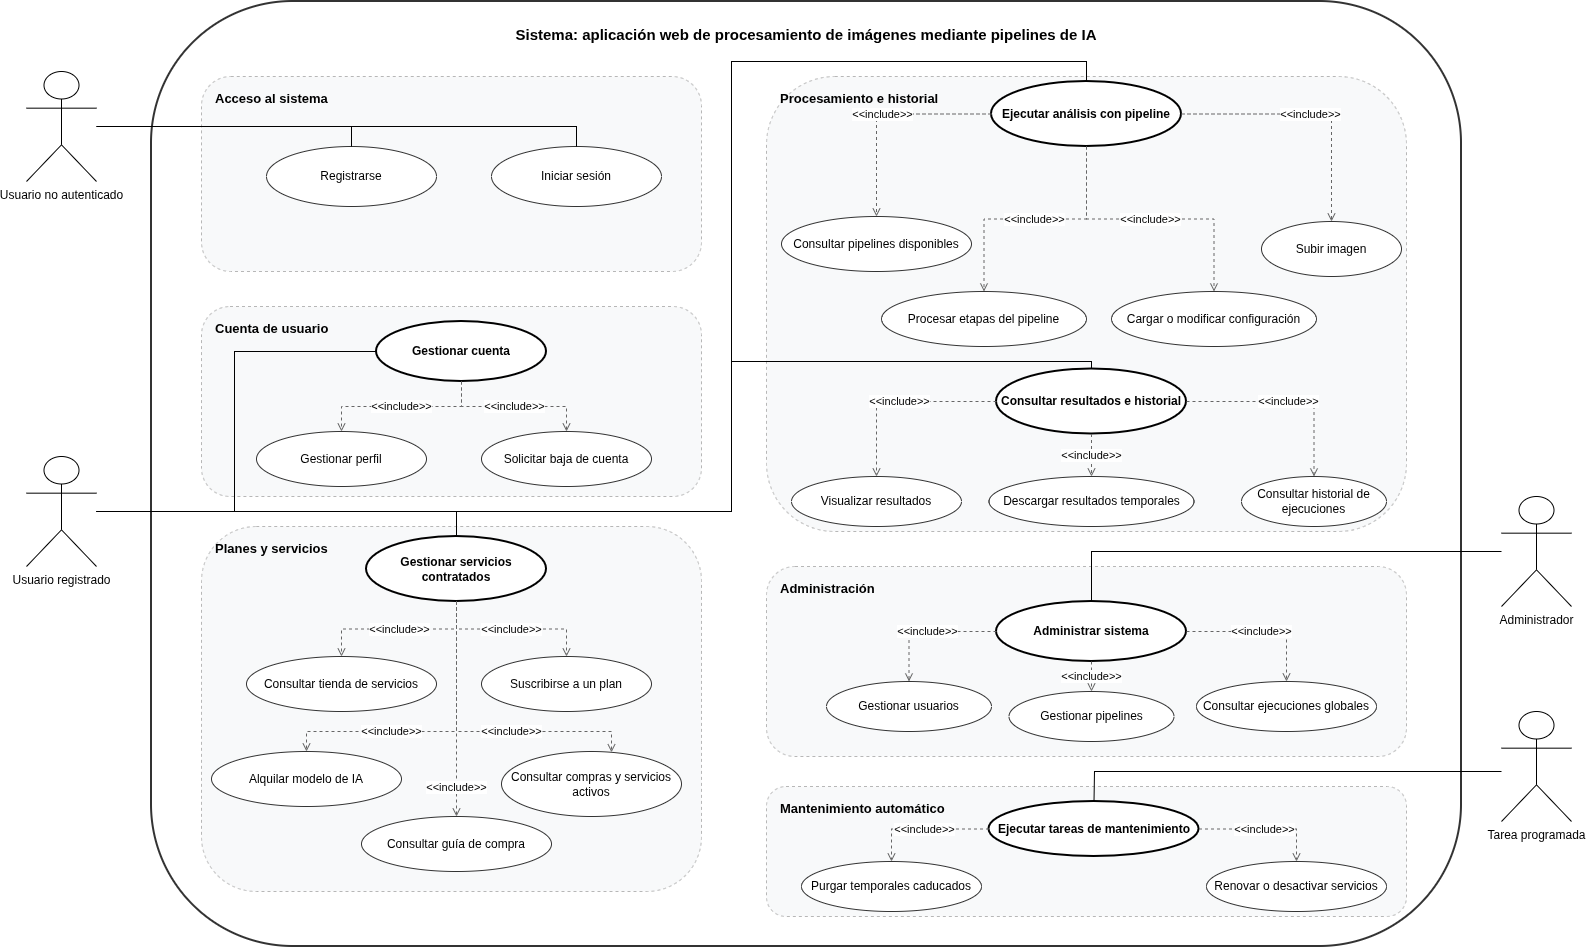
\includegraphics[width=0.95\textwidth]{img/diagrama_casos_uso.png}
	\caption[Diagrama de casos de uso del sistema]{Diagrama de casos de uso del sistema.}
	\label{fig:diagrama_casos_uso}
\end{figure}

El diagrama diferencia cuatro actores: usuario no autenticado, usuario registrado, administrador y sistema. El usuario no autenticado puede registrarse e iniciar sesión. El usuario registrado puede gestionar su cuenta, contratar servicios, consultar pipelines disponibles, ejecutar análisis sobre imágenes, visualizar resultados y consultar su historial. El administrador dispone de funciones de gestión de usuarios, pipelines y ejecuciones globales. Por último, el sistema representa las tareas automáticas de mantenimiento, como la limpieza de archivos temporales, renovación o desactivación de servicios y anonimización de cuentas dadas de baja.

A partir de esta visión general, se detallan a continuación los casos de uso identificados. Para cada uno de ellos se resume el actor principal, los requisitos asociados, la finalidad del caso de uso, sus precondiciones, el flujo principal, el resultado esperado y las posibles excepciones.


% Formato compacto para los casos de uso.
% Se usa xtabular para permitir división entre páginas y evitar espacios en blanco innecesarios.
\newenvironment{casouso}[2]{%
	\begingroup
	\small
	\renewcommand{\arraystretch}{1.08}
	\def\cuLabel{#2}
	\begin{center}
		\bottomcaption{#1.}
		\begin{xtabular}{@{}p{0.22\linewidth}p{0.70\linewidth}@{}}
			\toprule
		}{%
			\bottomrule
		\end{xtabular}
		\label{tabla:\cuLabel}
	\end{center}
	\endgroup
}

\begin{casouso}{CU-1 Registrarse}{cu1}
	\textbf{Actor} & Usuario no autenticado. \\
	\textbf{RF} & RF-1.1, RF-13.2. \\
	\textbf{Descripción} & Creación de una cuenta para acceder a las funciones privadas de la aplicación. \\
	\textbf{Precondición} & No existe una cuenta con el mismo correo o nombre de usuario. \\
	\textbf{Flujo principal} & El usuario accede al registro, introduce sus datos, el sistema valida los campos, comprueba duplicados, crea la cuenta y asigna el rol de usuario. \\
	\textbf{Resultado} & La cuenta queda creada y puede utilizarse para iniciar sesión. \\
	\textbf{Excepciones} & Correo duplicado, nombre de usuario duplicado, contraseña no válida o datos incompletos. \\
	\textbf{Importancia} & Alta. \\
\end{casouso}

\begin{casouso}{CU-2 Iniciar sesión}{cu2}
	\textbf{Actor} & Usuario. \\
	\textbf{RF} & RF-1.2, RF-2.1, RF-2.2, RF-13.2. \\
	\textbf{Descripción} & Acceso a la aplicación mediante credenciales válidas. \\
	\textbf{Precondición} & El usuario dispone de una cuenta activa. \\
	\textbf{Flujo principal} & El usuario introduce sus credenciales, el sistema las valida, comprueba el estado de la cuenta, genera el token de acceso y redirige al panel correspondiente. \\
	\textbf{Resultado} & El usuario queda autenticado en el sistema. \\
	\textbf{Excepciones} & Credenciales incorrectas, usuario inexistente o cuenta suspendida. \\
	\textbf{Importancia} & Alta. \\
\end{casouso}

\begin{casouso}{CU-3 Gestionar perfil}{cu3}
	\textbf{Actor} & Usuario. \\
	\textbf{RF} & RF-1.4, RF-1.5, RF-1.6, RF-13.4. \\
	\textbf{Descripción} & Consulta y modificación de los datos básicos de la cuenta. \\
	\textbf{Precondición} & El usuario ha iniciado sesión. \\
	\textbf{Flujo principal} & El usuario accede al perfil, consulta sus datos, modifica los campos permitidos y el sistema valida y guarda los cambios. Si cambia la contraseña, debe indicar la contraseña actual. \\
	\textbf{Resultado} & Los datos de la cuenta quedan actualizados. \\
	\textbf{Excepciones} & Contraseña actual incorrecta, nueva contraseña no válida o error de persistencia. \\
	\textbf{Importancia} & Media. \\
\end{casouso}

\begin{casouso}{CU-4 Solicitar baja de cuenta}{cu4}
	\textbf{Actor} & Usuario. \\
	\textbf{RF} & RF-1.7, RF-12.4. \\
	\textbf{Descripción} & Baja lógica de una cuenta y desactivación de sus servicios activos. \\
	\textbf{Precondición} & El usuario ha iniciado sesión. \\
	\textbf{Flujo principal} & El usuario solicita la baja, el sistema localiza la cuenta, la marca como borrada, desactiva sus servicios activos y registra la fecha de baja. \\
	\textbf{Resultado} & La cuenta queda dada de baja y sus servicios dejan de estar activos. \\
	\textbf{Excepciones} & Identidad no localizada o error al aplicar la baja. \\
	\textbf{Importancia} & Media. \\
\end{casouso}

\begin{casouso}{CU-5 Consultar tienda de servicios}{cu5}
	\textbf{Actor} & Usuario. \\
	\textbf{RF} & RF-3.1, RF-3.3, RF-13.5. \\
	\textbf{Descripción} & Consulta de planes y modelos disponibles para contratación. \\
	\textbf{Precondición} & El usuario ha iniciado sesión. \\
	\textbf{Flujo principal} & El usuario accede a la tienda, el sistema recupera los planes y modelos habilitados y muestra el estado de cada servicio respecto al usuario. \\
	\textbf{Resultado} & El usuario puede decidir qué plan o modelo contratar. \\
	\textbf{Excepciones} & Error al recuperar el catálogo de servicios. \\
	\textbf{Importancia} & Alta. \\
\end{casouso}

\begin{casouso}{CU-6 Suscribirse a un plan}{cu6}
	\textbf{Actor} & Usuario. \\
	\textbf{RF} & RF-3.2, RF-3.6, RF-3.7. \\
	\textbf{Descripción} & Contratación de un plan de servicio para ampliar el acceso a modelos y pipelines. \\
	\textbf{Precondición} & El usuario ha iniciado sesión y el plan está disponible. \\
	\textbf{Flujo principal} & El usuario selecciona un plan, el sistema comprueba su disponibilidad, registra la suscripción, define su vigencia y actualiza los permisos de acceso. \\
	\textbf{Resultado} & El usuario dispone del plan contratado. \\
	\textbf{Excepciones} & Plan inexistente, plan no disponible o error al registrar la suscripción. \\
	\textbf{Importancia} & Alta. \\
\end{casouso}

\begin{casouso}{CU-7 Alquilar un modelo de IA}{cu7}
	\textbf{Actor} & Usuario. \\
	\textbf{RF} & RF-3.3, RF-3.4, RF-3.6, RF-3.7. \\
	\textbf{Descripción} & Contratación individual de un modelo de IA para ejecutar pipelines que dependan de él. \\
	\textbf{Precondición} & El usuario ha iniciado sesión y el modelo está habilitado. \\
	\textbf{Flujo principal} & El usuario selecciona un modelo, el sistema comprueba que exista, que esté habilitado y que no exista ya un acceso activo, y registra el alquiler con su periodo de vigencia. \\
	\textbf{Resultado} & El usuario puede acceder a pipelines que utilicen el modelo contratado. \\
	\textbf{Excepciones} & Modelo inexistente, modelo ya contratado, fecha inválida o error de registro. \\
	\textbf{Importancia} & Alta. \\
\end{casouso}

\begin{casouso}{CU-8 Consultar compras y servicios activos}{cu8}
	\textbf{Actor} & Usuario. \\
	\textbf{RF} & RF-3.5, RF-3.6, RF-3.7, RF-13.5. \\
	\textbf{Descripción} & Consulta de planes, alquileres y servicios activos o programados. \\
	\textbf{Precondición} & El usuario ha iniciado sesión. \\
	\textbf{Flujo principal} & El usuario accede a sus compras, el sistema recupera sus suscripciones y alquileres, muestra fechas, estado y renovación automática, y permite modificar las opciones admitidas. \\
	\textbf{Resultado} & El usuario conoce el estado de sus servicios. \\
	\textbf{Excepciones} & Error al recuperar la información o intento de modificar un servicio inexistente. \\
	\textbf{Importancia} & Media-alta. \\
\end{casouso}

\begin{casouso}{CU-9 Consultar guía de compra}{cu9}
	\textbf{Actor} & Usuario. \\
	\textbf{RF} & RF-4.6, RF-13.6. \\
	\textbf{Descripción} & Consulta orientativa de los modelos o planes necesarios para ejecutar cada pipeline. \\
	\textbf{Precondición} & El usuario ha iniciado sesión. \\
	\textbf{Flujo principal} & El usuario accede a la guía, el sistema obtiene los pipelines y sus modelos requeridos, indica qué requisitos cumple el usuario y qué servicios tendría que contratar. \\
	\textbf{Resultado} & El usuario dispone de información para decidir qué servicio contratar. \\
	\textbf{Excepciones} & No existen pipelines disponibles o se produce un error al calcular dependencias. \\
	\textbf{Importancia} & Media. \\
\end{casouso}

\begin{casouso}{CU-10 Consultar pipelines disponibles}{cu10}
	\textbf{Actor} & Usuario. \\
	\textbf{RF} & RF-4.3, RF-4.4, RF-4.5, RF-13.3. \\
	\textbf{Descripción} & Obtención de los pipelines ejecutables según rol, plan y modelos contratados. \\
	\textbf{Precondición} & El usuario ha iniciado sesión. \\
	\textbf{Flujo principal} & El usuario accede al panel principal, el sistema identifica su cuenta, revisa sus permisos y muestra únicamente los pipelines que puede ejecutar. \\
	\textbf{Resultado} & El usuario puede seleccionar un pipeline permitido. \\
	\textbf{Excepciones} & Si no hay pipelines disponibles, se muestra un aviso y se deshabilita la ejecución. \\
	\textbf{Importancia} & Muy alta. \\
\end{casouso}

\begin{casouso}{CU-11 Cargar y modificar configuración del pipeline}{cu11}
	\textbf{Actor} & Usuario. \\
	\textbf{RF} & RF-5.1, RF-5.2, RF-5.3, RF-5.4, RF-5.5. \\
	\textbf{Descripción} & Consulta y edición de la configuración de ejecución de un pipeline. \\
	\textbf{Precondición} & El usuario ha seleccionado un pipeline permitido. \\
	\textbf{Flujo principal} & El usuario solicita la configuración, el sistema recupera la configuración predeterminada de las etapas, la interfaz la muestra en formato editable y el usuario puede modificarla antes de ejecutar. \\
	\textbf{Resultado} & La configuración queda preparada para utilizarse en la ejecución. \\
	\textbf{Excepciones} & Configuración no encontrada, JSON incorrecto o pipeline no permitido. \\
	\textbf{Importancia} & Alta. \\
\end{casouso}

\begin{casouso}{CU-12 Ejecutar pipeline sobre una imagen}{cu12}
	\textbf{Actor} & Usuario. \\
	\textbf{RF} & RF-6.1, RF-6.2, RF-6.3, RF-6.4, RF-6.5, RF-6.6, RF-6.7. \\
	\textbf{Descripción} & Flujo principal de procesamiento de una imagen mediante un pipeline. \\
	\textbf{Precondición} & El usuario ha iniciado sesión y tiene acceso al pipeline seleccionado. \\
	\textbf{Flujo principal} & El usuario selecciona un pipeline, adjunta una imagen, ajusta opcionalmente la configuración y lanza el análisis. El sistema valida imagen, configuración y permisos, ejecuta las etapas, registra la ejecución y devuelve los resultados. \\
	\textbf{Resultado} & La ejecución queda registrada y el usuario puede visualizar los resultados generados. \\
	\textbf{Excepciones} & Archivo inválido, pipeline no permitido, configuración incorrecta, error de procesamiento o ausencia de resultados útiles. \\
	\textbf{Importancia} & Muy alta. \\
\end{casouso}

\begin{casouso}{CU-13 Visualizar y descargar resultados}{cu13}
	\textbf{Actor} & Usuario. \\
	\textbf{RF} & RF-7.1, RF-7.2, RF-7.3, RF-7.4, RF-7.5, RF-9.2. \\
	\textbf{Descripción} & Visualización y descarga temporal de resultados generados por una ejecución. \\
	\textbf{Precondición} & Existe una ejecución completada con archivos disponibles. \\
	\textbf{Flujo principal} & El sistema muestra las etapas, imágenes y datos JSON generados. El usuario puede descargar los archivos disponibles y el sistema resuelve la descarga mediante tokens temporales. \\
	\textbf{Resultado} & El usuario visualiza o descarga los resultados mientras estén disponibles. \\
	\textbf{Excepciones} & Archivo caducado, token inválido, archivo eliminado físicamente o acceso no autorizado. \\
	\textbf{Importancia} & Alta. \\
\end{casouso}

\begin{casouso}{CU-14 Consultar historial de ejecuciones}{cu14}
	\textbf{Actor} & Usuario. \\
	\textbf{RF} & RF-8.1, RF-8.2, RF-8.3, RF-8.4, RF-8.5, RF-13.7. \\
	\textbf{Descripción} & Consulta de ejecuciones realizadas por el usuario autenticado. \\
	\textbf{Precondición} & El usuario ha iniciado sesión. \\
	\textbf{Flujo principal} & El usuario accede al historial, el sistema recupera sus ejecuciones y muestra pipeline, fecha, estado, duración y errores. Si selecciona una ejecución, se muestran sus detalles y archivos disponibles. \\
	\textbf{Resultado} & El usuario puede revisar sus ejecuciones y resultados temporales disponibles. \\
	\textbf{Excepciones} & No existen ejecuciones, ejecución no encontrada o intento de acceder a una ejecución ajena. \\
	\textbf{Importancia} & Alta. \\
\end{casouso}

\begin{casouso}{CU-15 Acceder al panel de administración}{cu15}
	\textbf{Actor} & Administrador. \\
	\textbf{RF} & RF-2.3, RF-2.5, RF-10.1, RF-13.8. \\
	\textbf{Descripción} & Acceso del administrador a la consola de gestión del sistema. \\
	\textbf{Precondición} & El usuario ha iniciado sesión con rol de administrador. \\
	\textbf{Flujo principal} & El administrador inicia sesión, el sistema detecta su rol, lo redirige al panel de administración y muestra las secciones de gestión disponibles. \\
	\textbf{Resultado} & El administrador puede acceder a funciones de revisión y gestión. \\
	\textbf{Excepciones} & Usuario no administrador o token no válido. \\
	\textbf{Importancia} & Alta. \\
\end{casouso}

\begin{casouso}{CU-16 Gestionar usuarios desde administración}{cu16}
	\textbf{Actor} & Administrador. \\
	\textbf{RF} & RF-10.2, RF-10.3, RF-10.4, RF-10.5. \\
	\textbf{Descripción} & Consulta de usuarios y modificación controlada de su estado. \\
	\textbf{Precondición} & El administrador ha accedido al panel de administración. \\
	\textbf{Flujo principal} & El administrador consulta los usuarios, selecciona una cuenta, solicita un cambio de estado y el sistema valida y aplica la operación. \\
	\textbf{Resultado} & El estado de la cuenta queda actualizado. \\
	\textbf{Excepciones} & Usuario no encontrado, intento de auto-bloqueo o error al actualizar la base de datos. \\
	\textbf{Importancia} & Alta. \\
\end{casouso}

\begin{casouso}{CU-17 Gestionar pipelines desde administración}{cu17}
	\textbf{Actor} & Administrador. \\
	\textbf{RF} & RF-11.1, RF-11.2, RF-11.3, RF-11.4, RF-11.5, RF-11.6, RF-11.7, RF-11.8. \\
	\textbf{Descripción} & Creación, modificación, deshabilitación o eliminación de pipelines desde administración. \\
	\textbf{Precondición} & El administrador ha iniciado sesión y existen modelos y modos registrados. \\
	\textbf{Flujo principal} & El administrador consulta el catálogo, crea o selecciona un pipeline, define sus etapas y el sistema valida que los modelos y modos sean coherentes y estén habilitados antes de guardar los cambios. \\
	\textbf{Resultado} & El catálogo de pipelines queda actualizado sin modificar el código fuente. \\
	\textbf{Excepciones} & Pipeline inexistente, etapas inválidas, modelo o modo deshabilitado, falta de permisos o historial asociado que impida el borrado físico. \\
	\textbf{Importancia} & Muy alta. \\
\end{casouso}

\begin{casouso}{CU-18 Consultar ejecuciones globales}{cu18}
	\textbf{Actor} & Administrador. \\
	\textbf{RF} & RF-12.1, RNF-7. \\
	\textbf{Descripción} & Consulta administrativa del histórico general de ejecuciones del sistema. \\
	\textbf{Precondición} & El administrador ha accedido al panel de administración. \\
	\textbf{Flujo principal} & El administrador solicita la vista global, el sistema obtiene las ejecuciones registradas y muestra usuario, pipeline, fecha, estado, duración y errores. \\
	\textbf{Resultado} & El administrador dispone de una visión global del uso del sistema. \\
	\textbf{Excepciones} & Falta de permisos o error al obtener la información. \\
	\textbf{Importancia} & Media-alta. \\
\end{casouso}

\begin{casouso}{CU-19 Ejecutar tareas de mantenimiento}{cu19}
	\textbf{Actor} & Sistema. \\
	\textbf{RF} & RF-9.4, RF-9.5, RF-12.2, RF-12.3, RF-12.4. \\
	\textbf{Descripción} & Revisión de temporales, servicios caducados, renovaciones automáticas y cuentas dadas de baja. \\
	\textbf{Precondición} & Existen ejecuciones, servicios o cuentas susceptibles de revisión. \\
	\textbf{Flujo principal} & El sistema comprueba archivos temporales, elimina o invalida recursos caducados, revisa servicios vencidos, renueva o desactiva accesos y anonimiza cuentas dadas de baja cuando corresponda. \\
	\textbf{Resultado} & El sistema conserva un estado coherente y evita acumulación de recursos innecesarios. \\
	\textbf{Excepciones} & Si una tarea falla, no debe interrumpir el funcionamiento principal de la aplicación. \\
	\textbf{Importancia} & Alta. \\
\end{casouso}